% Options for packages loaded elsewhere
\PassOptionsToPackage{unicode}{hyperref}
\PassOptionsToPackage{hyphens}{url}
%
\documentclass[
  ignorenonframetext,
  aspectratio=169,
  aspectratio=169]{beamer}
\usepackage{pgfpages}
\usepackage{fontspec}
\usepackage{xeCJK}
\setmainfont{STHeiti}
\setsansfont{STHeiti} % 设置无衬线字体
\setmonofont{STHeiti}
\setCJKmainfont{STHeiti}  % 使用华文黑体作为中文字体
\setCJKsansfont{STHeiti}
\setCJKmonofont{STHeiti}
\usepackage{graphicx}
\usepackage{hyperref}
\usepackage{grffile} 

% 定义 \tightlist 命令
\providecommand{\tightlist}{%
  \setlength{\itemsep}{0pt}\setlength{\parskip}{0pt}}

% 定义 \pandocbounded 命令
\newcommand{\pandocbounded}[1]{#1}

\setbeamertemplate{caption}[numbered]
\setbeamertemplate{caption label separator}{: }
\setbeamercolor{caption name}{fg=normal text.fg}
\beamertemplatenavigationsymbolsempty

% Generate Table of Contents
\AtBeginSection[]{
  \begin{frame}
    \frametitle{Table of Contents}
    \setcounter{tocdepth}{2}
    \tableofcontents[currentsection,currentsubsection,hideothersubsections]
  \end{frame}
}
\usepackage{lmodern}
\usepackage{amssymb,amsmath}
\usepackage{ifxetex,ifluatex}
\ifnum 0\ifxetex 1\fi\ifluatex 1\fi=0 % if pdftex
  \usepackage[T1]{fontenc}
  \usepackage[utf8]{inputenc}
  \usepackage{textcomp} % provide euro and other symbols
\else % if luatex or xetex
  \usepackage{unicode-math}
  \defaultfontfeatures{Scale=MatchLowercase}
  \defaultfontfeatures[\rmfamily]{Ligatures=TeX,Scale=1}
\fi
\usetheme[]{Frankfurt}
\usecolortheme{beaver}
\usefonttheme{professionalfonts}
% Use upquote if available, for straight quotes in verbatim environments
\IfFileExists{upquote.sty}{\usepackage{upquote}}{}
\IfFileExists{microtype.sty}{% use microtype if available
  \usepackage[]{microtype}
  \UseMicrotypeSet[protrusion]{basicmath} % disable protrusion for tt fonts
}{}
\makeatletter
\@ifundefined{KOMAClassName}{% if non-KOMA class
  \IfFileExists{parskip.sty}{%
    \usepackage{parskip}
  }{% else
    \setlength{\parindent}{0pt}
    \setlength{\parskip}{6pt plus 2pt minus 1pt}}
}{% if KOMA class
  \KOMAoptions{parskip=half}}
\makeatother
\usepackage{xcolor}
\definecolor{blanchedalmond}{rgb}{1.0, 0.92, 0.8}
\IfFileExists{xurl.sty}{\usepackage{xurl}}{} % add URL line breaks if available
\IfFileExists{bookmark.sty}{\usepackage{bookmark}}{\usepackage{hyperref}}
\hypersetup{
  pdftitle={My wonderful presentation},
  pdfauthor={Alexey Gumirov},
  hidelinks,
  pdfcreator={LaTeX via pandoc}}
\urlstyle{same} % disable monospaced font for URLs
\newif\ifbibliography
\usepackage{listings}
\newcommand{\passthrough}[1]{#1}
\lstset{defaultdialect=sh}
\lstset{framexleftmargin=0mm, frame=trBL,backgroundcolor=\color{blanchedalmond!5},numbers=left,numberstyle=\scriptsize,basicstyle=\small}
\lstset{aboveskip=5mm,belowskip=5mm,xleftmargin=20pt,xrightmargin=5pt}
% \lstset{prebreak={\raisebox{0ex}[0ex][0ex]}}
% \lstset{postbreak={\raisebox{0ex}[0ex][0ex]\space}}
\lstset{breaklines=true,breakatwhitespace=true}
\usepackage{longtable,booktabs}
\usepackage{caption}
% Make caption package work with longtable
\makeatletter
\def\fnum@table{\tablename~\thetable}
\makeatother
\usepackage{graphicx,grffile}
\makeatletter
\def\maxwidth{\ifdim\Gin@nat@width>\linewidth\linewidth\else\Gin@nat@width\fi}
\def\maxheight{\ifdim\Gin@nat@height>\textheight\textheight\else\Gin@nat@height\fi}
\makeatother
% Scale images if necessary, so that they will not overflow the page
% margins by default, and it is still possible to overwrite the defaults
% using explicit options in \includegraphics[width, height, ...]{}
\setkeys{Gin}{width=\maxwidth,height=\maxheight,keepaspectratio}
% Set default figure placement to htbp
\makeatletter
\def\fps@figure{htbp}
\makeatother
\usepackage[normalem]{ulem}
\newcommand{\st}[1]{\sout{#1}}
% Avoid problems with \sout in headers with hyperref
\pdfstringdefDisableCommands{\renewcommand{\sout}{}}
\setlength{\emergencystretch}{3em} % prevent overfull lines
\providecommand{\tightlist}{%
  \setlength{\itemsep}{0pt}\setlength{\parskip}{0pt}}
\setcounter{secnumdepth}{-\maxdimen} % remove section numbering

%
% When using babel or polyglossia with biblatex, loading csquotes is recommended 
% to ensure that quoted texts are typeset according to the rules of your main language.
%
\usepackage{csquotes}

%
% blockquote
%
\definecolor{blockquote-border}{RGB}{221,221,221}
\definecolor{blockquote-text}{RGB}{89,89,89}
\usepackage{mdframed}
\newmdenv[rightline=false,bottomline=false,topline=false,linewidth=3pt,linecolor=blockquote-border,skipabove=\parskip]{customblockquote}
\renewenvironment{quote}{\begin{customblockquote}\list{}{\rightmargin=0em\leftmargin=0em}%
\item\relax\color{blockquote-text}\ignorespaces}{\unskip\unskip\endlist\end{customblockquote}}

%
% Source Sans Pro as the de­fault font fam­ily
% Source Code Pro for monospace text
%
% 'default' option sets the default 
% font family to Source Sans Pro, not \sfdefault.
%
\usepackage[default]{sourcesanspro}
\usepackage{sourcecodepro}

% XeLaTeX specific adjustments for straight quotes: https://tex.stackexchange.com/a/354887
% This issue is already fixed (see https://github.com/silkeh/latex-sourcecodepro/pull/5) but the 
% fix is still unreleased.
% TODO: Remove this workaround when the new version of sourcecodepro is reelased on CTAN.
\ifxetex
\makeatletter
\defaultfontfeatures[\ttfamily]
  { Numbers   = \sourcecodepro@figurestyle,
    Scale     = \SourceCodePro@scale,
    Extension = .otf }
\setmonofont
  [ UprightFont    = *-\sourcecodepro@regstyle,
    ItalicFont     = *-\sourcecodepro@regstyle It,
    BoldFont       = *-\sourcecodepro@boldstyle,
    BoldItalicFont = *-\sourcecodepro@boldstyle It ]
  {SourceCodePro}
\makeatother
\fi


\title{My wonderful presentation}
\author{Alexey Gumirov}
\date{07 一月 2025}
\institute{My home office}
\titlegraphic{
\includegraphics{img/aleph0.png}}
\logo{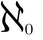
\includegraphics{img/aleph0-small.png}}

\begin{document}
\frame{\titlepage}

\begin{frame}
  \tableofcontents[hideallsubsections]
\end{frame}
\section{General information beamer}\label{general-information-beamer}

\subsection{Themes, fonts, etc. beamer}\label{themes-fonts-etc.-beamer}

\begin{frame}{Themes, fonts, etc. beamer}
\begin{itemize}
\tightlist
\item
  I use default \textbf{pandoc} themes.
\item
  This presentation is made with \textbf{Frankfurt} theme and
  \textbf{beaver} color theme.
\item
  I like \textbf{professionalfonts} font scheme.
\end{itemize}
\end{frame}

\subsection{Links beamer}\label{links-beamer}

\begin{frame}{Links beamer}
\begin{itemize}
\tightlist
\item
  Matrix of beamer themes:
  \url{https://hartwork.org/beamer-theme-matrix/}
\item
  Font themes:
  \href{http://www.deic.uab.es/~iblanes/beamer_gallery/index_by_font.html}{http://www.deic.uab.es/\textasciitilde iblanes/beamer\emph{gallery/index}by\_font.html}
\item
  Nerd Fonts: \url{https://nerdfonts.com}
\end{itemize}
\end{frame}

\section{Formatting beamer}\label{formatting-beamer}

\subsection{Text formatting beamer}\label{text-formatting-beamer}

\begin{frame}{Text formatting beamer}
Normal text. \emph{Italic text} and \textbf{bold text}. \st{Strike out}
is supported.
\end{frame}

\subsection{Notes beamer}\label{notes-beamer}

\begin{frame}{Notes beamer}
\begin{quote}
This is a note.

\begin{quote}
Nested notes are not supported. And it continues.
\end{quote}
\end{quote}
\end{frame}

\subsection{Blocks}\label{blocks}

\begin{frame}{This is a block A}
\phantomsection\label{this-is-a-block-a}
\begin{itemize}
\tightlist
\item
  Line A
\item
  Line B
\end{itemize}
\end{frame}

\begin{frame}{}
\phantomsection\label{section}
New block without header.
\end{frame}

\begin{frame}{This is a block B. beamer}
\phantomsection\label{this-is-a-block-b.-beamer}
\begin{itemize}
\tightlist
\item
  Line C
\item
  Line D
\end{itemize}
\end{frame}

\subsection{Listings}\label{listings}

\begin{frame}[fragile]{Listings}
Listings out of the block.

\begin{lstlisting}[language=sh]
#!/bin/bash
echo "Hello world!"
echo "line"
\end{lstlisting}
\end{frame}

\begin{frame}[fragile]{Listings in the block. beamer}
\phantomsection\label{listings-in-the-block.-beamer}
\begin{lstlisting}[language=sh]
#!/bin/bash
echo "Hello world!"
echo "line"
\end{lstlisting}
\end{frame}

\subsection{Table beamer}\label{table-beamer}

\begin{frame}{Table beamer}
\begin{longtable}[]{@{}lrc@{}}
\toprule\noalign{}
\textbf{Item} & \textbf{Description} & \textbf{Q-ty} \\
\midrule\noalign{}
\endhead
Item A & Item A description & 2 \\
Item B & Item B description & 5 \\
Item C & N/A & 100 \\
\bottomrule\noalign{}
\end{longtable}
\end{frame}

\subsection{Single picture}\label{single-picture}

\begin{frame}[fragile]{Single picture}
This is how we insert picture. Caption is produced automatically from
the alt text.

\begin{lstlisting}
![Aleph 0](img/aleph0.png) 
\end{lstlisting}

\begin{figure}
\centering

\includegraphics{img/aleph0.png}
\caption{Aleph 0}
\end{figure}
\end{frame}

\subsection{Two or more pictures in a
raw}\label{two-or-more-pictures-in-a-raw}

\begin{frame}{Two or more pictures in a raw}
Here are two pictures in the raw. We can also change two pictures size
(height or width).
\end{frame}

\begin{frame}[fragile]{}
\phantomsection\label{section-1}
\begin{lstlisting}
![](img/aleph0.png){height=10%}\ ![](img/aleph0.png){height=30%} 
\end{lstlisting}


\includegraphics[width=\textwidth,height=0.1\textheight]{img/aleph0.png}~
\includegraphics[width=\textwidth,height=0.3\textheight]{img/aleph0.png}
\end{frame}

\subsection{Lists}\label{lists}

\begin{frame}{Lists}
\begin{enumerate}
\tightlist
\item
  Idea 1
\item
  Idea 2

  \begin{itemize}
  \tightlist
  \item
    genius idea A
  \item
    more genius 2
  \end{itemize}
\item
  Conclusion
\end{enumerate}
\end{frame}

\subsection{Two columns of equal
width}\label{two-columns-of-equal-width}

\begin{frame}{Two columns of equal width}
\begin{columns}[T]
\begin{column}{0.48\textwidth}
Left column text.

Another text line.
\end{column}

\begin{column}{0.48\textwidth}
\begin{itemize}
\tightlist
\item
  Item 1.
\item
  Item 2.
\item
  Item 3.
\end{itemize}
\end{column}
\end{columns}
\end{frame}

\subsection{Two columns of with 40:60
split}\label{two-columns-of-with-4060-split}

\begin{frame}{Two columns of with 40:60 split}
\begin{columns}[T]
\begin{column}{0.4\textwidth}
Left column text.

Another text line.
\end{column}

\begin{column}{0.6\textwidth}
\begin{itemize}
\tightlist
\item
  Item 1.
\item
  Item 2.
\item
  Item 3.
\end{itemize}
\end{column}
\end{columns}
\end{frame}

\subsection{Three columns with equal
split}\label{three-columns-with-equal-split}

\begin{frame}{Three columns with equal split}
\begin{columns}[T]
\begin{column}{0.48\textwidth}
Left column text.

Another text line.
\end{column}

\begin{column}{0.48\textwidth}
Middle column list:

\begin{enumerate}
\tightlist
\item
  Item 1.
\item
  Item 2.
\end{enumerate}
\end{column}

\begin{column}{0.48\textwidth}
Right column list:

\begin{itemize}
\tightlist
\item
  Item 1.
\item
  Item 2.
\end{itemize}
\end{column}
\end{columns}
\end{frame}

\subsection{Three columns with 30:40:30
split}\label{three-columns-with-304030-split}

\begin{frame}{Three columns with 30:40:30 split}
\begin{columns}[T]
\begin{column}{0.3\textwidth}
Left column text.

Another text line.
\end{column}

\begin{column}{0.4\textwidth}
Middle column list:

\begin{enumerate}
\tightlist
\item
  Item 1.
\item
  Item 2.
\end{enumerate}
\end{column}

\begin{column}{0.3\textwidth}
Right column list:

\begin{itemize}
\tightlist
\item
  Item 1.
\item
  Item 2.
\end{itemize}
\end{column}
\end{columns}
\end{frame}

\subsection{Two columns: image and
text}\label{two-columns-image-and-text}

\begin{frame}{Two columns: image and text}
\begin{columns}[T]
\begin{column}{0.48\textwidth}

\includegraphics[width=\textwidth,height=0.5\textheight]{img/aleph0.png}
\end{column}

\begin{column}{0.48\textwidth}
Text in the right column.

List from the right column:

\begin{itemize}
\tightlist
\item
  Item 1.
\item
  Item 2.
\end{itemize}
\end{column}
\end{columns}
\end{frame}

\subsection{Two columns: image and
table}\label{two-columns-image-and-table}

\begin{frame}{Two columns: image and table}
\begin{columns}[T]
\begin{column}{0.48\textwidth}

\includegraphics[width=\textwidth,height=0.5\textheight]{img/aleph0.png}
\end{column}

\begin{column}{0.48\textwidth}
\begin{longtable}[]{@{}lc@{}}
\toprule\noalign{}
\textbf{Item} & \textbf{Option} \\
\midrule\noalign{}
\endhead
Item 1 & Option 1 \\
Item 2 & Option 2 \\
\bottomrule\noalign{}
\end{longtable}
\end{column}
\end{columns}
\end{frame}

\subsection{Fancy layout beamer}\label{fancy-layout-beamer}

\begin{frame}{Proposal}
\phantomsection\label{proposal}
\begin{itemize}
\tightlist
\item
  Point A
\item
  Point B
\end{itemize}
\end{frame}

\begin{columns}[T]
\begin{column}{0.48\textwidth}
\begin{frame}{Pros}
\phantomsection\label{pros}
\begin{itemize}
\tightlist
\item
  Good
\item
  Better
\item
  Best
\end{itemize}
\end{frame}
\end{column}

\begin{column}{0.48\textwidth}
\begin{frame}{Cons beamer}
\phantomsection\label{cons-beamer}
\begin{itemize}
\tightlist
\item
  Bad
\item
  Worse
\item
  Worst
\end{itemize}
\end{frame}
\end{column}
\end{columns}

\begin{frame}{Conclusion beamer}
\phantomsection\label{conclusion-beamer}
\begin{itemize}
\tightlist
\item
  Let's go for it!
\item
  No way we go for it!
\end{itemize}
\end{frame}

\end{document}
